%\documentclass[a4paper,english,12pt,twocolumn]{article}
\documentclass[a4paper,english,12pt]{article}
\usepackage[utf8]{inputenc} % Encodage du fichier
\usepackage[T1]{fontenc} % Encodage des fonts nécessaire pour le Latin
\usepackage[french]{babel} % Pour changer la langue des mots générés et choisir la bonne mise en page
\usepackage{amssymb}
\usepackage{pdflscape}
\usepackage{microtype} 
\usepackage{lmodern} % Le latin modèrne
\usepackage[top=2cm, bottom=2cm, left=2.5cm, right=1.5cm]{geometry} % Définir les marges de la page 
\usepackage[hidelinks,urlcolor=blue,unicode=true,
pdftitle={Multi-armed bandits},
pdfauthor={BELOUADAH Eden},
pdfdisplaydoctitle=true]{hyperref} % Pour les liens 
\usepackage{fancyhdr} % Pour le style de la page
\usepackage[font=it]{caption} % Rendre les titres des tableaux italiques
\usepackage{graphicx} % Pour les images
\usepackage{subcaption} % Pour mettre plusieurs images sur la même ligne
\usepackage{float} % Pour empêcher le déplacement des tableaux et des figures.
\usepackage{babelbib} % Pour changer la langue dans la bibliographie
\usepackage{amsmath} % Pour des fonctions mathématiques
\usepackage{amssymb} % Pour les symboles mathématiques
%\usepackage[onelanguage,english,longend,boxruled,algoruled,linesnumbered,algochapter,nofillcomment]{algorithm2e} %pour les algorithmes
\usepackage{multirow}
\usepackage{booktabs}
\usepackage{enumitem}
\usepackage{setspace}

\graphicspath{ {images/} } % Spécifier le répertoire contenant les images

\DisableLigatures[f]{encoding=*}

%Active ça si tu ne veux pas les points-virgules dans les algorithmes
% \DontPrintSemicolon
 
%\renewcommand \thechapter{\Roman{chapter}} % Utiliser les numéros romans pour les chapitres

\captionsetup{labelfont=it,textfont=it,labelsep=period} % Changer le style des légendes
\AtBeginDocument{ % Changer les légendes
	\renewcommand\tablename{\itshape Tableau}
	\renewcommand{\figurename}{\itshape Figure}
	% Renommer la table des matières
	\renewcommand{\contentsname}{Sommaire}
}

% Style de l'entête et le pied de la page
\setlength{\headheight}{-70pt}
\pagestyle{fancy}
\fancyhead[L]{} % Enlever la section
\fancyhead[R]{\footnotesize\slshape{\nouppercase{\leftmark}}} % Titre du chapitre en minuscule avec taille 10
\fancyfoot[C]{}
\fancyfoot[R]{\thepage} % Déplacer le numéro de la page vers la droite de la page

\fancypagestyle{plain}{
\renewcommand{\headrulewidth}{0pt}
\fancyhf{}
\fancyfoot[R]{\thepage}
}
  
% Espace entre les lignes
\linespread{1.3}

% Code pris de https://tex.stackexchange.com/a/95616/109916 et corrigé
% Début
\makeatletter
\newcommand{\emptypage}[1]{
  \cleardoublepage
  \begingroup
  \let\ps@plain\ps@empty
  \pagestyle{empty}
  #1
  \cleardoublepage
  \endgroup}
\makeatletter
% Fin


% pour changer les deux points des légendes d'algorithmes
% \SetAlgoCaptionSeparator{\unskip.}

\begin{document}
%\include{Page_de_garde}
%\include{Remerciements}
\emptypage{
%\tableofcontents
%\listoffigures
%\listoftables
}
    
\setlength{\parskip}{0.6em plus 0.1em minus 0.1em}
%\SetKwInput{KwOut}{Outpits}

% Redéfinition des chapitres et sections pour les inclure dans le sommaire
\makeatletter
%	\let\oldchapter\chapter
%	\newcommand{\@chapterstar}[1]{\cleardoublepage\phantomsection\addcontentsline{toc}{chapter}{#1}{\oldchapter*{#1}}\markboth{#1}{}}
%	\newcommand{\@chapternostar}[1]{{\oldchapter{#1}}}
%	\renewcommand{\chapter}{\@ifstar{\@chapterstar}{\@chapternostar}}
\let\oldsection\section
\newcommand{\@sectionstar}[1]{\phantomsection\addcontentsline{toc}{section}{#1}{\oldsection*{#1}}}
\newcommand{\@sectionnostar}[1]{{\oldsection{#1}}}
\renewcommand\section{\@ifstar{\@sectionstar}{\@sectionnostar}}	
\newcommand*{\rom}[1]{\expandafter\@slowromancap\romannumeral #1@}
\makeatother

\setcounter{page}{1}
%%%%%%%%%%%%%%%%%%%%%%%%%%%%%%%%%%%%%%%%%%%%%%%%%%%%%%%%%%%%%

\title{Multi-armed bandits}
\author{Eden BELOUADAH}
\date{}
\maketitle

\section{Introduction}
Le but de ce travail pratique est d'implémenter plusieurs bandits à bras multiples et voir la différence entre eux.

\section{Bandits à plusieurs bras}
Un bandit à plusieurs bras est un agent qui a $K$ bras et à chaque pas de temps, il essaye de choisir un bras de telle manière à faire un compromis entre l'exploration et l'exploitation. Le but étant de minimiser le regret total après un certain horizon de temps T.
\subsection{Agent $\epsilon$-greedy}
Cet agent choisit à chaque fois avec une probabilité d'exploitation $1-\epsilon$ le bras ayant la moyenne de récompenses la plus grande depuis le début de la partie, et avec une probabilité d'exploration $\epsilon$, un bras aléatoire uniformément choisi.
\vspace{-1em}
$$
i_t=argmax\{\hat{\mu}_{1,t},\hat{\mu}_{2,t},...,\hat{\mu}_{k,t}\} 
$$
\vspace{-1em}
Les résultats obtenus sont les suivants:

\begin{figure}[H]
	\centering
	\begin{subfigure}{0.48\textwidth}
		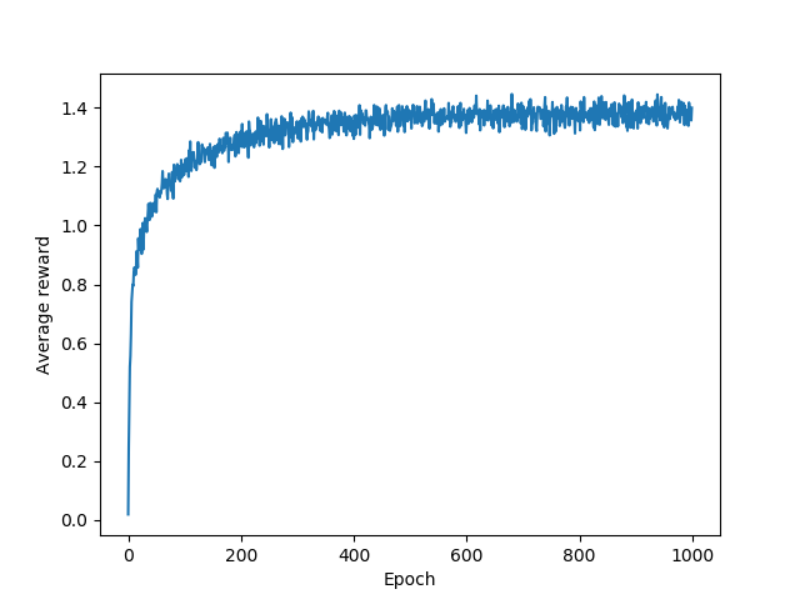
\includegraphics[width=\textwidth]{eps_reward}
		\caption{Évolution des récompenses}
	\end{subfigure}
	\begin{subfigure}{0.48\textwidth}
		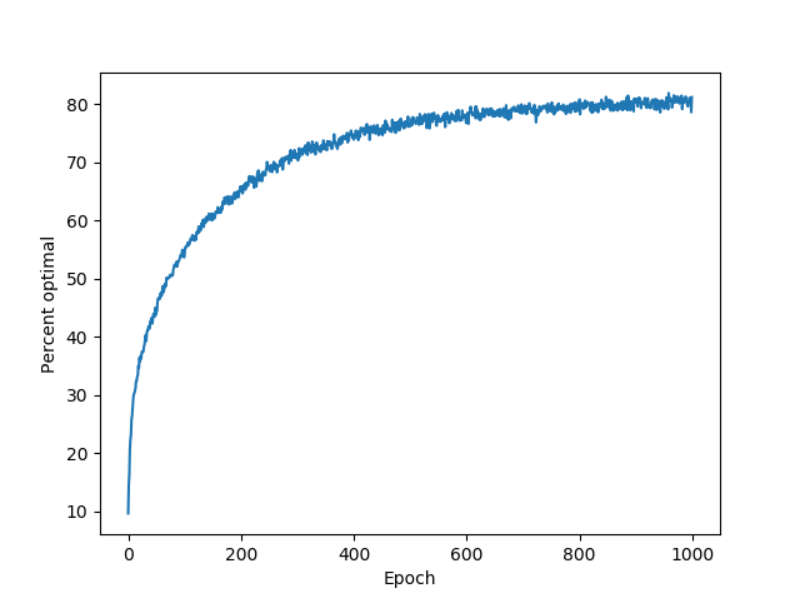
\includegraphics[width=\textwidth]{eps_optimal}
		\caption{Évolution de l'optimum}
	\end{subfigure}
	\caption{Résultats obtenus pour l'agent $\epsilon$-greedy}
\end{figure}
\vspace{-1em}

\subsection{Agent Optimistic $\epsilon$-greedy}
Cet agent est le même que le précédent, sauf qu'il initialise les Q\_valeurs de chaque bras non pas à 0 mais à une valeur appelée $optimism$. Les résultats obtenus sont les suivats:

\begin{figure}[H]
	\centering
	\begin{subfigure}{0.48\textwidth}
		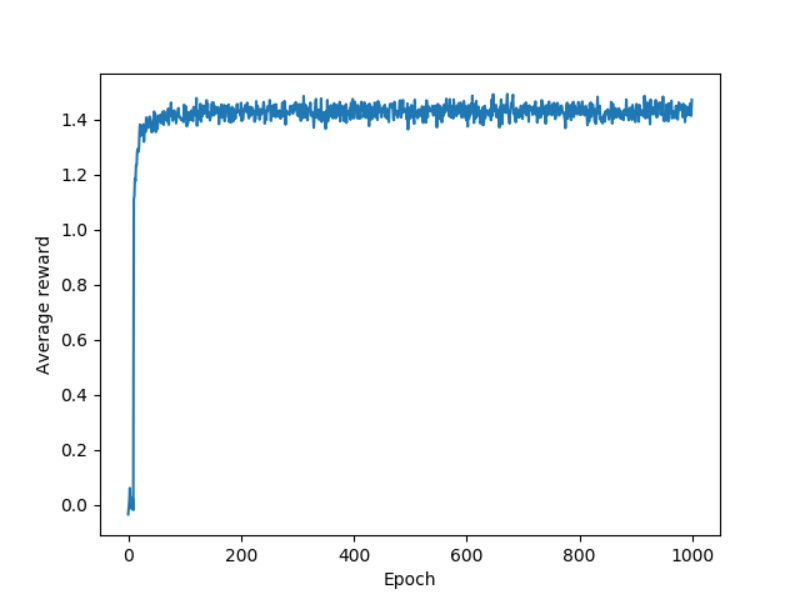
\includegraphics[width=\textwidth]{opt_reward}
		\caption{Évolution des récompenses}
	\end{subfigure}
	\begin{subfigure}{0.48\textwidth}
		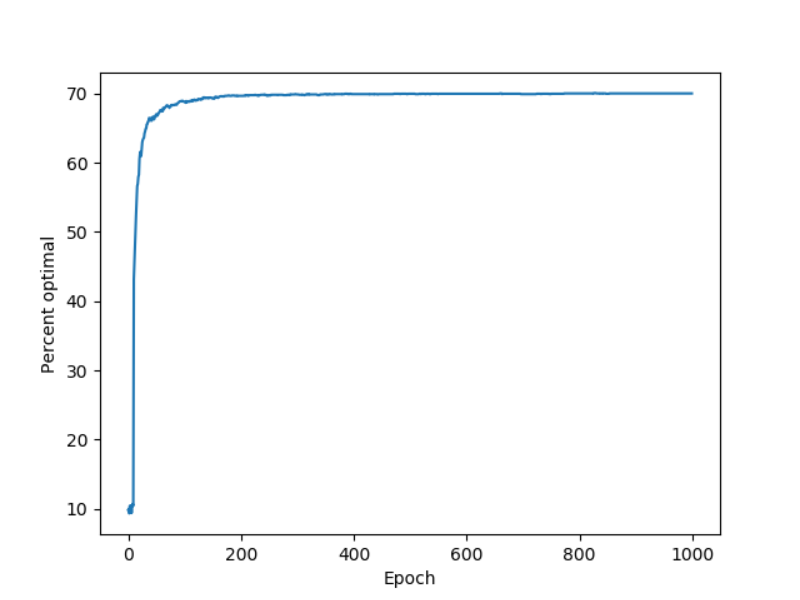
\includegraphics[width=\textwidth]{opt_optimal}
		\caption{Évolution de l'optimum}
	\end{subfigure}
	\caption{Résultats obtenus pour l'agent Optimistic $\epsilon$-greedy}
\end{figure}

Nous remarquons que l'initialisation des Q\_valeurs des bras a un grand impact sur la qualité de l'agent. En effet, la récompense fait un saut énorme vers des valeurs optimales peut perturbées au début de l'exécution. 

\subsection{Agent SoftMax}

\vspace{-0.5em}
Cet agent choisit à chaque itération un bras avec une probabilité ($\tau$ est la température) :

\vspace{-1.5em}
$$
p_k=\frac{e^{\frac{\hat{\mu}_k}{\tau}}}{\sum_{i=1}^{k}e^{\frac{\hat{\mu}_i}{\tau}}}
$$
Les résultats obtenus sont les suivants:
\begin{figure}[H]
	\centering
	\begin{subfigure}{0.48\textwidth}
		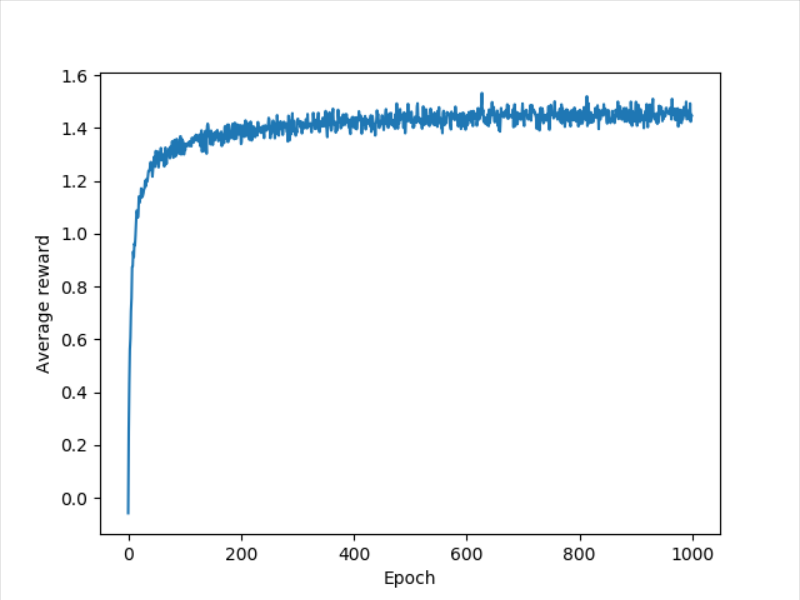
\includegraphics[width=\textwidth]{soft_reward}
		\caption{Évolution des récompenses}
	\end{subfigure}
	\begin{subfigure}{0.48\textwidth}
		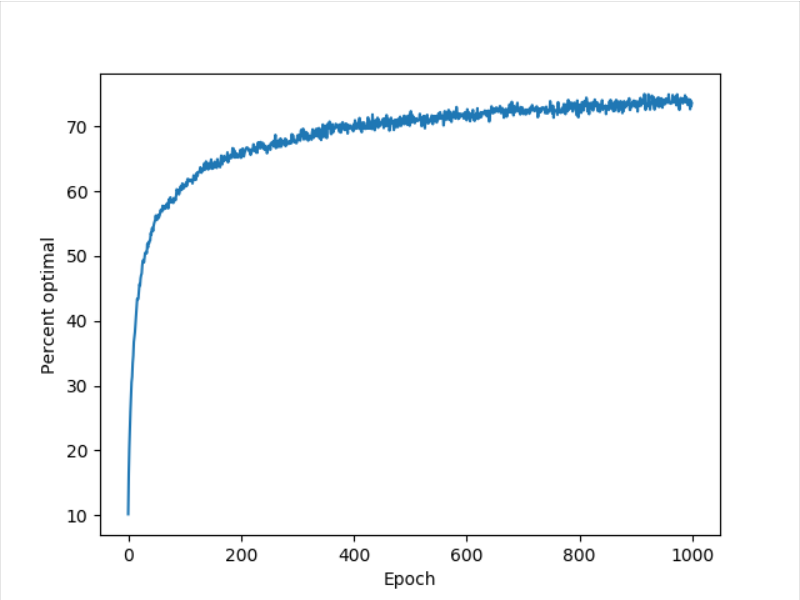
\includegraphics[width=\textwidth]{soft_optimal}
		\caption{Évolution de l'optimum}
	\end{subfigure}
	\caption{Résultats obtenus pour l'agent SoftMax}
\end{figure}

\vspace{-1.5em}
Nous remarquons que la récompense de l'agent augmente rapidement et ensuite elle est moins perturbée que celle de l'agent $\epsilon$-greedy.

\vspace{-1em}
\subsection{Agent UCB (Upper Confidence Bound)}

\vspace{-0.5em}
Cet agent choisit le bras maximisant la moyenne des récompenses plus l'intervalle de confiance ($n_{i,t}$ est le nombre de fois où le bras $i$ a été choisi du début jusqu'à l'instant $t$):

\vspace{-1.5em}
$$
i_t=argmax\{\hat{\mu}_{i,t}+\sqrt{2 \frac{Log(\sum n_{j,t})}{n_{i,t}}}\}
$$

\vspace{-1em}
Les résultats obtenus sont les suivants:

\begin{figure}[H]
	\centering
	\begin{subfigure}{0.48\textwidth}
		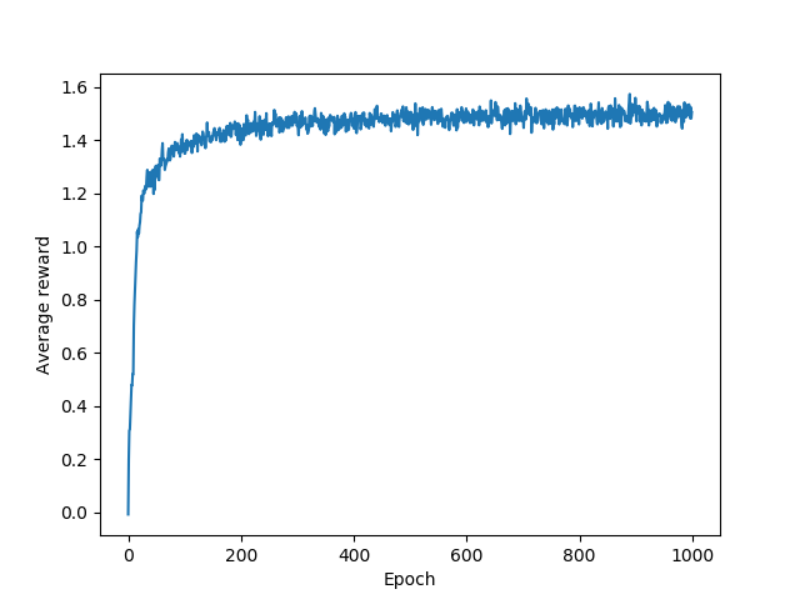
\includegraphics[width=\textwidth]{ucb_reward}
		\caption{Évolution des récompenses}
	\end{subfigure}
	\begin{subfigure}{0.48\textwidth}
		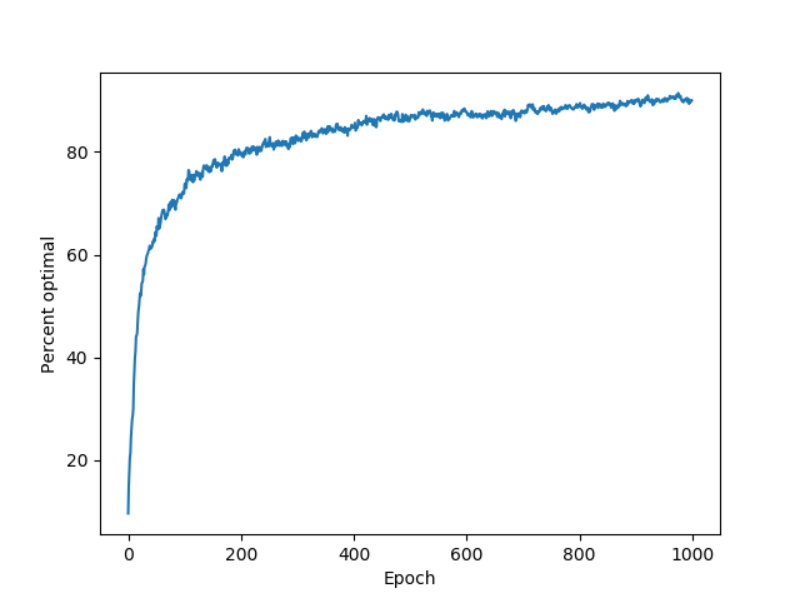
\includegraphics[width=\textwidth]{ucb_optimal}
		\caption{Évolution de l'optimum}
	\end{subfigure}
	\caption{Résultats obtenus pour l'agent Thompson}
\end{figure}

De même, nous remarquons que la récompense de l'agent augmente rapidement et presque de la même façon que celle de l'agent SoftMax. De plus, l'évolution dans l'optimum est meilleure et plus stable.

\subsection{Agent Thompson}

Cet agent échantillonne selon la loi normale et choisit le meilleur bras comme suit:

$$
i_t=argmax\{\mathcal{N}(\hat{\mu}_{i,t},\frac{1}{n_{i,t}+1})\}
$$

Les résultats obtenus sont les suivants:
\begin{figure}[H]
	\centering
	\begin{subfigure}{0.48\textwidth}
		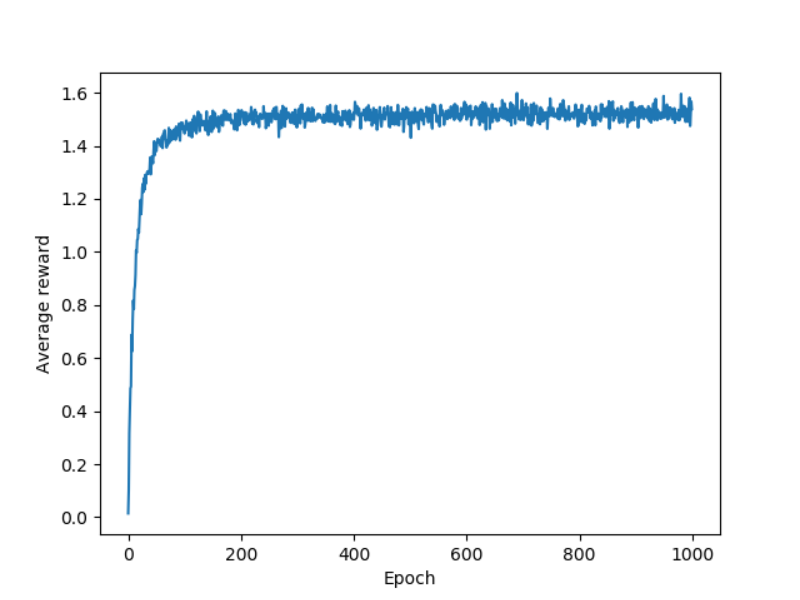
\includegraphics[width=\textwidth]{thomps_reward}
		\caption{Évolution des récompenses}
	\end{subfigure}
	\begin{subfigure}{0.48\textwidth}
		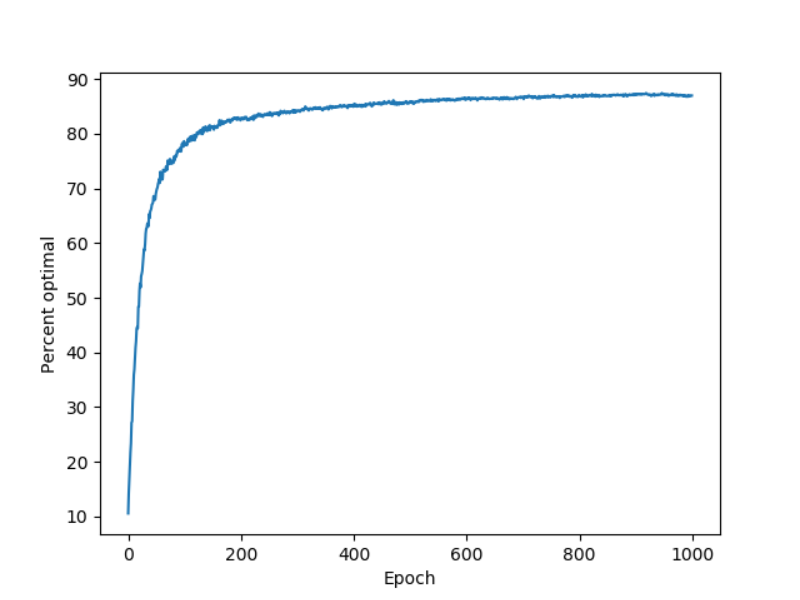
\includegraphics[width=\textwidth]{thomps_optimal}
		\caption{Évolution de l'optimum}
	\end{subfigure}
	\caption{Résultats obtenus pour l'agent Thompson}
\end{figure}

Les résultats pour cet agent sont les meilleurs, la récompense continue à augmenter jusqu'à arriver à de très grande valeurs non perturbées.

\section{Conclusion}
En comparant le temps d'exécution des agent, on trouve:

\begin{table}[H]\centering
	\begin{tabular}{cccccc}
		\toprule \textbf{Agent} & $\epsilon$-greedy & Optimistic $\epsilon$-greedy & SoftMax & UCB & Thompson\\    \midrule
		\textbf{Temps d'exécution(s)} & 20.52 & 24.02& 189.29 & 60.25 & 37.40  \\   
		\bottomrule	
	\end{tabular}
	\caption{Temps d'exécution des bandits}
\end{table}

Nous remarquons que l'agent le plus rapide est $\epsilon$-greedy (avec les deux versions simple et optimiste) vu qu'il est naïf et n'effectue aucun traitement particulier à part la comparaison avec la probabilité d'exploration $\epsilon$.

En revanche, l'agent le plus lent est SoftMax, et cela parce qu'il calcule à chaque itération l'exponentiel de la fraction de la moyenne des récompenses par la température pour tous les bras afin de pouvoir calculer la probabilité de choisir chaque bras.

Les deux agents UCB et Thompson sont plus ou moins rapides. 







%%%%%%%%%%%%%%%%%%%%%%%%%%%%%%%%%%%%%%%%%%%%%%%%%%%%%%%%%%%%%
\bibliographystyle{babplain}
\parskip=-1em
%\emptypage{\bibliography{bibliographie}}
\let\section\oldsection % pour éviter que le résumé soient visibles dans le sommaire comme une section
%\include{Resume}
\end{document}
